\documentclass[twoside,a4paper,11pt]{article}
\setlength{\oddsidemargin}{0.25 in}
\setlength{\evensidemargin}{-0.25 in}
\setlength{\topmargin}{-0.6 in}
\setlength{\textwidth}{6.5 in}
\setlength{\textheight}{8.5 in}
\setlength{\headsep}{0.75 in}
\setlength{\parindent}{0 in}
\setlength{\parskip}{0.1 in}

%
% ADD PACKAGES here:
%
\usepackage[utf8]{inputenc} %for UTF8-extended encoding
\usepackage{amsmath,amsfonts,amssymb,graphicx,mathtools,flexisym}
\usepackage{caption} %for figures and labels captions
\usepackage{pbox} %to break the cell text in tables
\usepackage[skins,theorems]{tcolorbox} %to create color boxes for examples and recap

\usepackage[colorinlistoftodos,prependcaption,textsize=tiny]{todonotes}
\usepackage{tikz}
\usetikzlibrary{patterns,3d,calc}

\captionsetup{labelsep=space}
%
% The following commands set up the lecnum (lecture number)
% counter and make various numbering schemes work relative
% to the lecture number.
%
\newcounter{lecnum}
\renewcommand{\thepage}{\thelecnum-\arabic{page}}
\renewcommand{\thesection}{\thelecnum.\arabic{section}}
\renewcommand{\theequation}{\thelecnum.\arabic{equation}}
\renewcommand{\thefigure}{\thelecnum.\arabic{figure}}
\renewcommand{\thetable}{\thelecnum.\arabic{table}}

%
% The following macro is used to generate the header.
%
\newcommand{\lecture}[5]{
   \pagestyle{myheadings}
   \thispagestyle{plain}
   \newpage
   \setcounter{lecnum}{#1}
   \setcounter{page}{1}
   \noindent
   \begin{center}
   {\bf COVENTRY UNIVERSITY}
   \framebox{
      \vbox{\vspace{2mm}
    \hbox to 6.28in { {\bf 208MED: Mechanics
	\hfill Spring 2019} }
       \vspace{4mm}
       \hbox to 6.28in { {\Large \hfill Lecture #1: #2  \hfill} }
       \vspace{2mm}
       \hbox to 6.28in { {\textsl{#3} \hfill \texttt{#4}} }
      \vspace{2mm}}
   }
   \end{center}
   \markboth{Lecture #1: #2}{Lecture #1: #2}

%   {\bf Note}: {\it LaTeX template courtesy of UC Berkeley EECS dept.}

   {\bf Disclaimer}: {\it These notes have not been subjected to the
   usual scrutiny reserved for formal publications.  They may be distributed
   outside this class only with the permission of the instructor.}
   \vspace*{4mm}
}

% **** IF YOU WANT TO DEFINE ADDITIONAL MACROS FOR YOURSELF, PUT THEM HERE:


\begin{document}
%FILL IN THE RIGHT INFO.
%\lecture{**LECTURE-NUMBER**}{**DATE**}{**LECTURER**}{**SCRIBE**}
\lecture{02}{Properties of area and bending}{Dr. Arnaldo Delli-Carri}{ac4213@coventry.ac.uk}
%\footnotetext{These notes are partially based on those of R. C. Hibbeler}

\tableofcontents

% **** YOUR NOTES GO HERE:

\section{Properties of area}

\subsection{Centroid and first moments of area}
The position of the centroid of a plane area is an important geometric property. To obtain formulas for locating centroids, we will refer to Fig. \ref{fig:GenericSection} which shows a plane area of generic shape with its centroid at point $c$. The $xy$ coordinate system is oriented arbitrarily with its origin at any point $O$. The area of the geometric figure is defined by the following integral:

\begin{equation}
A=\int_A \,dA
\end{equation}

in which $dA$ is a differential element of area having coordinates $x$ and $y$ (Fig. \ref{fig:GenericSection}) and $A$ is the total area of the figure.

\begin{figure}[!htb]
	\centering
	\begin{tikzpicture}[scale=1]
	\draw[->] (-1,-1) -- +(4,0) node[right]{$\hat{x}$};
	\draw[->] (-1,-1) node[above right]{$O$} -- +(0,4) node[right]{$\hat{y}$};
	\draw[fill=cyan!50] plot [smooth cycle] coordinates {(0,0) (1,0.1) (2,0.3) (2,1.4) (1.5,2.5) (0.8,2.5) (0.3,1.2) (-0.2,0.6)};
	\fill (1.3,1.5) circle (2pt);
	\draw (1.3,1.5) node[above]{$c$};
	\draw[help lines,latex-latex] (1.3,-1) -- (1.3,1.5) node[pos=0.25,right]{$y_c$};
	\draw[help lines,latex-latex] (-1,1.5) -- (1.3,1.5) node[pos=0.3,above]{$x_c$};
	\draw[fill=cyan!60!black] (0.3,0.3) rectangle ++(0.3,0.3);
	\draw (0.6,0.6) node[above]{$dA$};
	\draw[help lines,latex-latex] (0.45,-1) -- (0.45,0.45) node[pos=0.25,right]{$y$};
	\draw[help lines,latex-latex] (-1,0.45) -- (0.45,0.45) node[pos=0.3,above]{$x$};
	
	\begin{scope}[xshift=6cm]
	\draw[->] (-1,-1) -- +(4,0) node[right]{$\hat{x}$};
	\draw[->] (-1,-1) node[above right]{$O$} -- +(0,4) node[right]{$\hat{y}$};
	\draw[fill=cyan!50] (0.5,-0.5) -- ++(0,2) -- ++(-1,0) -- ++(0,0.7) -- ++(3,0) -- ++(0,-0.7) -- ++(-1,0) -- ++(0,-2) -- cycle;
	\fill (1,1.2) circle (2pt);
	\draw (1,1.2) node[left]{$c$};
	\draw[dash pattern={on 7pt off 2pt on 1pt off 3pt}] (1,-0.9) -- ++(0,4);
	\draw[help lines] (1,1.2) -- ++(1.4,0);
	\draw[help lines,latex-latex] (2.2,-1) -- ++(0,2.2) node[pos=0.5,right]{$y_c$};
	\end{scope}
	
	\begin{scope}[xshift=12cm]
	\draw[->] (-1,-1) -- +(4,0) node[right]{$\hat{x}$};
	\draw[->] (-1,-1) node[above right]{$O$} -- +(0,4) node[right]{$\hat{y}$};
	\draw[fill=cyan!50] (0,-0.5) rectangle ++(2,3);
	\draw[fill=white]   (0.3,-0.2) rectangle (1.7,2.2);
	\fill (1,1) circle (2pt);
	\draw (1,1) node[above right]{$c$};
	\draw[dash pattern={on 7pt off 2pt on 1pt off 3pt}] (-0.9,1) -- ++(3.5,0);
	\draw[dash pattern={on 7pt off 2pt on 1pt off 3pt}] (1,-0.9) -- ++(0,4);
	\end{scope}
	\end{tikzpicture}
	\caption{Generic cross-section, one axis of symmetry, two axes of symmetry}
	\label{fig:GenericSection}
\end{figure}

The {\bf \emph{first moments of the area}} with respect to the $x$ and $y$ axes are defined, respectively, as follows:

\begin{equation}
I_x=\int_A y\,dA \qquad I_y=\int_A x\,dA
\end{equation}

Thus, the first moments represent the sums of the products of the differential areas and their coordinates. First moments may be positive or negative,
depending upon the position of the $xy$ axes. Also, first moments have units of length raised to the third power; for instance, $\text{mm}^3$. The coordinates $x_c$ and $y_c$ of the centroid $c$ (Fig. \ref{fig:GenericSection}) are equal to the first moments divided by the area:

\begin{equation}
x_c=\frac{\displaystyle \int_A y\,dA}{ \displaystyle \int_A\,dA} \qquad y_c=\frac{\displaystyle \int_A x\,dA}{\displaystyle \int_A\,dA}
\label{eq:FirstMomentIntegral}
\end{equation}

If the boundaries of the area are defined by simple mathematical expressions, we can evaluate the integrals appearing in Eq. \eqref{eq:FirstMomentIntegral} in closed form and thereby obtain formulas for $x_c$ and $y_c$. In general, the coordinates $x_c$ and $y_c$ may be positive or negative, depending upon the position of the centroid with respect to the reference axes. 

If an area is symmetric about an axis, the centroid must lie on that axis because the first moment about an axis of symmetry equals zero. For example, the centroid of the singly symmetric area shown in Fig. \ref{fig:GenericSection} must lie on the vertical axis of symmetry. Therefore, only the coordinate $y_c$ must be calculated in order to locate the centroid $c$. If an area has two axes of symmetry, as illustrated in Fig. \ref{fig:GenericSection}, the position of the centroid can be determined by inspection because it lies at the intersection of the axes of symmetry.

If an area has irregular boundaries not defined by simple mathematical expressions, we can locate the centroid by numerically evaluating the integrals in Eq. \eqref{eq:FirstMomentIntegral}. The simplest procedure is to divide the geometric figure into smaller sub-regions and replace the integrations with summations. If we denote the area of the $i$-th sub-region by $A_i$, then the expressions for the coordinates of the centroid are

\begin{equation}
x_c=\frac{\displaystyle \sum A_i x_i}{ \displaystyle \sum A_i} \qquad y_c=\frac{\displaystyle \sum A_i y_i}{ \displaystyle \sum A_i}
\label{eq:CentroidEquations}
\end{equation}

in which $x_i$ and $y_i$ are respectively the $x$ and $y$ coordinate of the centroid of the $i$-th sub-region. The accuracy of the calculations depends upon how closely the selected elements fit the actual area. If they fit exactly, the results are exact. Many computer programs for locating centroids use a numerical scheme similar to the one expressed by Eq. \eqref{eq:CentroidEquations}.

When using the formulas for composite areas, we can handle the \emph{absence} of an area by subtraction. This procedure is useful when there are cutouts or holes in the section. For instance, consider the area shown in Fig. \ref{fig:GenericSection}. We can analyze this figure as a composite area by subtracting the properties of the inner rectangle from the corresponding properties of the outer rectangle. (From another viewpoint, we can think of the outer rectangle as a "positive area" and the inner rectangle as a "negative area".) Similarly, if an area has a hole, we can subtract the properties of the area of the hole from those of the outer rectangle. (Again, the same effect is achieved if we treat the outer rectangle as a "positive area" and the hole as a "negative area".)

\subsection{Second moments of area}
The second moments of a plane area (also sometimes called \emph{moments of inertia of the area}) with respect to the $x$ and $y$ axes, respectively, are defined by the integrals 

\begin{equation}
I_{xx}=\int_A y^2\,dA \qquad I_{yy}=\int_A x^2\,dA
\label{eq:SecMomAreas}
\end{equation}

in which $x$ and $y$ are the coordinates of the differential element of area $dA$. It is trivial to see that second moments of areas (unlike first moments) are always positive quantities and they are measured in units that are the fourth power of a length (e.g. $\text{mm}^4$).

\begin{figure}[hbt]
	\centering
	\begin{tikzpicture}[scale=1]
	\draw[->] (-1,-1) -- +(4,0) node[right]{$\hat{x}$};
	\draw[->] (-1,-1) node[above right]{$O$} -- +(0,4) node[right]{$\hat{y}$};
	\draw[fill=cyan!50] plot [smooth cycle] coordinates {(0,0) (1,0.1) (2,0.3) (2,1.4) (1.5,2.5) (0.8,2.5) (0.3,1.2) (-0.2,0.6)};
	\fill (1.3,1.5) circle (2pt);
	\draw (1.3,1.5) node[above]{$c$};
	\draw[fill=cyan!60!black] (0.3,0.3) rectangle ++(0.3,0.3);
	\draw (0.6,0.6) node[above]{$dA$};
	\draw[help lines,latex-latex] (0.45,-1) -- (0.45,0.45) node[pos=0.25,right]{$y$};
	\draw[help lines,latex-latex] (-1,0.45) -- (0.45,0.45) node[pos=0.3,above]{$x$};
	
	\begin{scope}[xshift=6cm,yshift=-0.5cm]	
	\draw[fill=cyan!50] (0,0) rectangle ++(2,3);
	\draw[fill=cyan!50!black] (0,2.3) rectangle ++(2,0.3) node[below left,xshift=-0.5,yshift=-0.3cm,black]{$dA$};
	\fill (1,1.5) circle (2pt);
	\draw (1,1.5) node[below left]{$c$};
	\draw[->] (-1,1.5) -- +(4,0) node[right]{$\hat{x}$};
	\draw[->] (1,-0.5) -- +(0,4.5) node[right]{$\hat{y}$};
	\draw (-1,0) node[above]{$n$} -- +(4,0) node[above]{$n$};
	\draw[help lines,latex-latex] (0,-0.4) -- ++(1,0) node[fill=white,midway]{$\frac{b}{2}$};
	\draw[help lines,latex-latex] (1,-0.4) -- ++(1,0) node[fill=white,midway]{$\frac{b}{2}$};
	\draw[help lines,latex-latex] (-0.4,0) -- ++(0,1.5) node[fill=white,midway]{$\frac{h}{2}$};
	\draw[help lines,latex-latex] (-0.4,1.5) -- ++(0,1.5) node[fill=white,midway]{$\frac{h}{2}$};
	\draw[help lines,latex-latex] (2.2,2.3) -- ++(0,0.3) node[midway,right]{$dy$};
	\draw[help lines,-latex] (2.2,1.5) -- (2.2,2.3) node[midway,right]{$y$};
	\end{scope}
	
	\begin{scope}[xshift=12cm,yshift=-0.5cm]
	\draw[fill=cyan!50] (0,0) rectangle ++(2,3);
	\draw[fill=white] (0.3,0.3) rectangle ++(1.4,2.4);
	\fill (1,1.5) circle (2pt);
	\draw (1,1.5) node[above right]{$c$};
	\draw[->] (1,1.5) -- +(2,0) node[right]{$\hat{x}$};
	\draw[->] (1,1.5) -- +(0,2.5) node[right]{$\hat{y}$};
	\draw[help lines,latex-latex] (0,-0.4) -- ++(2,0) node[fill=white,midway]{$H$};
	\draw[help lines,latex-latex] (-0.4,0) -- ++(0,3) node[fill=white,midway]{$B$};
	\draw[help lines,latex-latex] (0.3,0.7) -- ++(1.4,0) node[fill=white,midway]{$b$};
	\draw[help lines,latex-latex] (0.6,0.3) -- ++(0,2.4) node[fill=white,midway]{$h$};
	\end{scope}
	\end{tikzpicture}
	\caption{Generic cross-section, rectangular cross-section, boxed cross-section}
	\label{fig:SecMomArea}
\end{figure}

To illustrate how second moments of area are obtained by integration, we will consider a rectangle having width $b$ and height $h$ like in Fig. \ref{fig:SecMomArea}. The $x$ and $y$ axes have their origin at the centroid $c$. For convenience, we use a differential element of area $dA$ in the form of a thin horizontal strip of width $b$ and height $dy$ (therefore, $dA=b\cdot dy$ ). Since all parts of the elemental strip are the same distance from the $x$ axis, we can express the second moment of area $I_{xx}$ with respect to the $x$ axis as follows: 


\begin{equation}
I_{xx}=\int_A y^2\,dA=\int\limits_{-h/2}^{h/2}y^2\cdot b\,dy=b\left[\frac{y^3}{3}\right]_{-h/2}^{h/2}=\frac{bh^3}{12}
\end{equation}

In a similar manner, we can use an element of area in the form of a vertical strip with area and obtain the second moment of area with respect to the $y$ axis: 


\begin{equation}
I_{yy}=\int_A x^2\,dA=\int\limits_{-b/2}^{b/2}x^2\cdot h\,dx=h\left[\frac{x^3}{3}\right]_{-b/2}^{b/2}=\frac{hb^3}{12}
\end{equation}


If a different set of axes is selected, the second moments of area will have different values. For instance, consider axis $n-n$ at the base of the rectangle in Fig. \ref{fig:SecMomArea}. If this axis is selected as the reference, we must define $y$ as the coordinate distance from that axis to the element of area $dA$. Then the calculation for the second moment of area becomes


\begin{equation}
I_{nn}=\int_A y^2\,dA=\int_{0}^{h}y^2\cdot b\,dy=b\left[\frac{y^3}{3}\right]_{0}^{h}=\frac{bh^3}{3}
\label{eq:Inn}
\end{equation}

Note that the second moment of area with respect to axis $n-n$ is larger than the second moment of area with respect to the centroidal $x$ axis. In general, the second moment of area increases as the reference axis is moved parallel to itself farther from the centroid. 

The second moment of area of a composite area with respect to any particular axis is the sum of the second moments of area of its parts \emph{with respect to that same axis}. An example is the hollow boxed section shown in Fig. \ref{fig:SecMomArea}, where the $x$ and $y$ axes are axes of symmetry through the centroid $c$. The second moment of area $I_{xx}$ with respect to the $x$ axis is equal to the algebraic sum of the second moments of area of the outer and inner rectangles. As explained earlier, we can think of the inner rectangle as a "negative area" and the outer rectangle as a "positive area", therefore

\begin{equation}
I_{xx}=\frac{BH^3}{12}-\frac{bh^3}{12}
\end{equation}

Some known formulae for second moments of area are listed in Table xxx. For shapes not shown, the second moments of area can usually be obtained by using the listed formulas in conjunction with the parallel-axis theorem. If an area is of such irregular shape that its second moments of area cannot be obtained in this manner, then we can use numerical methods. The procedure is to divide the area into small elements of area $A_i$, multiply each such area by the square of its distance from the reference axis, and then sum the products.

\subsection{Parallel axis theorem}
In this section we will derive a very useful theorem pertaining to second moments of areas. Known as the {\bf \emph{parallel-axis theorem}}, it gives the relationship between the second moment of area with respect to a centroidal axis and the second moment of area with respect to any parallel axis. 

To derive the theorem, we consider an area of arbitrary shape with centroid $c$ (Fig. \ref{eq:SecMomAreas}a). We also consider two sets of coordinate axes: the axes with origin at the centroid, and a set of parallel $xy$ axes with origin at any point $O$. The distances between the two sets of parallel axes are denoted $d_1$ and $d_2$. Also, we identify an element of area $dA$ having coordinates $x$ and $y$ with respect to the centroidal axes. From the definition of second moment of area, we can write the following equation for the second moment of area $I_{xx}$ with respect to the $x$ axis: 

\begin{equation}
I_{xx}=\int_A (y+d_1)^2\,dA=\left(\int_A y^2\,dA\right) + \left(2d_1\int_A y\,dA\right) + \left(d_1^2\int_A\,dA\right)
\end{equation}

The first integral on the right-hand side is the second moment of area with respect to the $x_c$ axis. The second integral is the first moment of the area with respect to the $x_c$ axis (this integral equals zero because the $x_c$ axis passes through the centroid). The third integral is the area $A$ itself. Therefore, the preceding equation reduces to (and similarly for the axis $y$ with respect to the axis $y_c$)

\begin{equation}
I_{xx}=I_{x_cx_c}+A\cdot d_1^2 \qquad I_{yy}=I_{y_cy_c}+A\cdot d_2^2
\label{eq:ParallelAxisTheorem}
\end{equation}


Equations \eqref{eq:ParallelAxisTheorem} represent the parallel-axis theorem for second moments of area: \emph{the second moment of area with respect to any axis in its plane is equal to the second moment of area with respect to a parallel centroidal axis plus the product of the area and the square of the distance between the two axes.}

To illustrate the use of the theorem, consider again the rectangle shown in Fig. \ref{eq:SecMomAreas}b. Knowing that the second moment of area about the $x$ axis, which is through the centroid, is $I_{xx}=bh^3/12$, we can determine the second moment of area $I_{nn}$ about the base of the rectangle by using the parallel-axis theorem: 

\begin{equation}
I_{nn}=I_{xx}+A\cdot d_1^2 =\frac{bh^3}{12}+bh\cdot \left(\frac{h}{2}\right)^2=\frac{bh^3}{3}
\end{equation}

This result agrees with the second moment of area obtained previously by integration in Eq. \eqref{eq:Inn}. From the parallel-axis theorem, we see that the second moment of area increases as the axis is moved parallel to itself farther from the centroid. Therefore, the second moment of area about a centroidal axis is the least second moment of area (for a given direction of the axis). When using the parallel-axis theorem, it is essential to remember that one of the two parallel axes \emph{must} be a centroidal axis.

\subsection{Radius of gyration}
A distance known as the {\bf \emph{radius of gyration}} is occasionally encountered in mechanics. Radius of gyration of a plane area is defined as the square root of the second moment of area divided by the area itself; thus, 

\begin{equation}
\rho_x=\sqrt{\dfrac{I_{xx}}{A}} \qquad \rho_y=\sqrt{\dfrac{I_{yy}}{A}}
\end{equation}

in which $\rho_x$ and $\rho_y$ denote the radii of gyration with respect to the $x$ and $y$ axes, respectively. Since the second moment of area has units of length to the fourth power and area has units of length to the second power, radius of gyration has units of length (e.g $\text{mm}$). Although the radius of gyration of an area does not have an obvious physical meaning, we may consider it to be the distance (from the reference axis) at which the entire area could be concentrated and still have the same second moment of area as the original area.

\subsection{Polar moments of area}
The moments of area discussed in the preceding sections are defined with respect to axes lying in the plane of the area itself, such as the $x$ and $y$ axes in Fig. \ref{eq:SecMomAreas}. Now we will consider an axis \emph{perpendicular} to the plane of the area and intersecting the plane at the origin $O$. The moment of area with respect to this perpendicular axis is called the {\bf \emph{polar moment of area}} and is denoted by the symbol $J$. The polar moment of area with respect to an axis through $O$ perpendicular to the plane of the figure is defined by the integral

\begin{equation}
J_O=\int_A \rho^2\,dA
\end{equation}

in which $\rho$ is the distance from point $O$ to the differential element of area $dA$. This integral is similar in form to those for second moments of area $I_{xx}$ and $I_{yy}$ in Eq. \eqref{eq:FirstMomentIntegral}. Given that for Pythagora's theorem $\rho^2=x^2+y^2$, where $x$ and $y$ are the rectangular coordinates of the element $dA$, we obtain the following expression for $J_O$:

\begin{equation}
J_O=\int_A \rho^2\,dA=\int_A (x^2+y^2)\,dA=\int_A x^2\,dA+\int_A y^2\,dA
\end{equation}


Thus, we obtain the important relationship

\begin{equation}
J_O=I_{xx}+I_{yy}
\label{eq:PolarMoment}
\end{equation}

This equation shows that the polar moment of area with respect to an axis perpendicular to the plane of the figure at any point $O$ is equal to the sum of the second moments of area with respect to any two perpendicular axes $x$ and $y$ passing through that same point and lying in the plane of the figure. For convenience, we usually refer to $J_O$ simply as the polar moment of area with respect to point $O$, without mentioning that the axis is perpendicular to the plane of the figure. Also, to distinguish them from polar moments of area, we sometimes refer to $I_{xx}$ and $I_{yy}$ as rectangular moments of area. 

\begin{figure}[hbt]
	\centering
	\begin{tikzpicture}[scale=1]
	\draw[->] (-1,-1) -- +(4,0) node[right]{$\hat{x}$};
	\draw[->] (-1,-1) node[above left]{$O$} -- +(0,4) node[right]{$\hat{y}$};
	\draw[fill=cyan!50] plot [smooth cycle] coordinates {(0,0) (1,0.1) (2.1,0.3) (2.8,1.4) (2,2.5) (0.9,2.5) (0.3,1.2) (-0.2,0.6)};
	\draw[->] (1,1.1) -- +(2,0) node[right]{$x_c$};
	\draw[->] (1,1.1) -- +(0,1.9) node[right]{$y_c$};
	\fill (1,1.1) circle (2pt);
	\draw (1,1.1) node[above left]{$c$};
	\draw[fill=cyan!60!black] (1.6,1.6) rectangle ++(0.2,0.2);
	\draw (1.8,1.8) node[above,xshift=0.1cm]{$dA$};
	\draw[thin,latex-latex] (1.7,1.1) -- (1.7,1.6) node[pos=0.5,right]{$y$};
	\draw[thin,latex-latex] (1.1,1.7) -- (1.6,1.7) node[pos=0.5,above]{$x$};
	\draw[help lines,latex-latex] (-1,2.3) -- (1,2.3) node[pos=0.5,above]{$d_2$};
	\draw[help lines,latex-latex] (2.3,-1) -- (2.3,1.1) node[pos=0.5,right]{$d_1$};
	\draw[help lines,-latex] (-1,-1) -- (1,1.1) node[pos=0.4,xshift=-0.1cm,left]{$d$};
	
	\begin{scope}[xshift=7cm,yshift=1cm]
	\draw[fill=cyan!50] (0,0) circle (2cm);
	\draw[fill=cyan!50!black] (0,0) circle (1.5cm);
	\draw[fill=cyan!50] (0,0) circle (1.2cm);
	\fill (0,0) circle (2pt); \draw (0,0) node[above right]{$c$};
	\draw[->] (0,0) -- +(2.2,0) node[right]{$x_c$};
	\draw[->] (0,0) -- +(0,2.2) node[right]{$y_c$};
	\draw[thin,-latex] (0,0) -- ++(250:2cm) node[pos=0.3,left]{$r$};
	\draw[thin,-latex] (0,0) ++(-70:0.8cm) -- ++(-70:0.4cm) node[pos=0,right]{$dr$};
	\draw[thin,latex-] (0,0) ++(-70:1.5cm) -- ++(-70:0.4cm);
	\fill (-30:2cm) circle (2pt); \draw (-30:2cm) node[below right]{$P$};
	\end{scope}
	\end{tikzpicture}
	\caption{Generic cross-section, round cross-section}
	\label{fig:PolMomArea}
\end{figure}


Polar moments of area with respect to various points in the plane are related by the parallel-axis theorem for polar moments of area. We can derive this theorem by referring again to Fig. 12-13. Let us denote the polar moments of area with respect to the origin $O$ and the centroid $c$ by $J_O$ and $J_c$, respectively. Then, using Eq. \eqref{eq:PolarMoment}, we can write the following equations: 

\begin{equation}
J_O=I_{xx}+I_{yy} \qquad J_c=I_{x_cx_c}+I_{y_cy_c}
\end{equation}

Now refer to the parallel-axis theorems derived in the previous section for rectangular moments of area Eq. \eqref{eq:ParallelAxisTheorem}. Adding those two equations, we get

\begin{equation}
I_{xx}+I_{yy} = I_{x_cx_c}+I_{y_cy_c}+ A(d_1^2+d_2^2)
\end{equation}

now, noting that $d^2=d_1^2+d_2^2$ we obtain

\begin{equation}
J_O=J_c+A\cdot d^2
\end{equation}

This equation represents the parallel-axis theorem for polar moments of area:
\emph{the polar moment of area with respect to any point $O$ in its plane is equal to the polar moment of area with respect to the centroid $c$ plus the product of the area and the square of the distance between points $O$ and $C$.}

To illustrate the determination of polar moments of area and the use of the parallel-axis theorem, consider a circle of radius $r$ like in Fig. \ref{fig:PolMomArea}b. Let us take a differential element of area $dA$ in the form of a thin ring of radius $\rho$ and thickness $d\rho$ (thus, $dA=2\pi\rho\cdot d\rho$ ). Since every point in the element is at the same distance from the center of the circle, the polar moment of area of the entire circle with respect to the center is 

\begin{equation}
J_c=\int_A \rho^2\,dA=\int_0^r 2\pi\rho^3\,d\rho=2\pi\left[\frac{\rho^4}{4}\right]_0^r=\frac{\pi r^4}{2}=\frac{\pi D^4}{32}
\end{equation}

This result is also listed in Table xxx. The polar moment of area of the circle with respect to any point B on its circumference (Fig. 12-18) can be obtained from the parallel-axis
theorem: 

\begin{equation}
J_P=J_c+A\cdot d^2=\frac{\pi r^4}{2}+\pi r^2 \cdot r^2=\frac{3\pi r^4}{2}=\frac{3\pi D^4}{32}
\end{equation}


As an incidental matter, note that the polar moment of area has its smallest value when the reference point is the centroid of the area. A circle is a special case in which the polar moment of area can be determined by integration. However, most of the shapes encountered in engineering work do not lend themselves to this technique. Instead, polar moments of area are usually obtained by summing the rectangular moments of area for two perpendicular axes \ref{eq:PolarMoment}.

\section{Bending}
Members that are slender and support loadings that are applied perpendicular to their longitudinal axis are called \emph{beams}. In general, beams are long, straight bars having a constant cross-sectional area. Often they are classified as to how they are supported. For example, a simply supported beam is pinned at one end and roller supported at the other, Fig. \ref{fig:SimplyCantilever}a, a cantilevered beam is fixed at one end and free at the other, Fig \ref{fig:SimplyCantilever}b. 

\begin{figure}[hbt]
	\centering
	\begin{tikzpicture}[scale=1]
		\draw[fill=lightgray] (0,0) rectangle (5,0.4);
		\fill[black] (0,0) -- ++(-60:0.5) -- ++(180:0.5) -- cycle;
		\fill[black] (5,-0.2) circle (0.2cm);
	
	\begin{scope}[xshift=8cm]
		\draw[fill=lightgray] (0,0) rectangle (5,0.4);
		\fill[black] (-0.3,-0.3) rectangle (0,0.7);
	\end{scope}
	\end{tikzpicture}
	\caption{Simply supported beam (left) and cantilever beam (right)}
	\label{fig:SimplyCantilever}
\end{figure}

Beams are considered among the most important of all structural elements. They are used to support the floor of a building, the deck of a bridge, or the wing of an aircraft. Also, the axle of an automobile, the boom of a crane, even many of the bones of the body act as beams.

Because of the applied loadings, beams develop an internal shear force and bending moment that, in general, vary from point to point along the axis of the beam. In order to properly design a beam it therefore becomes important to determine the maximum shear and moment in the beam. One way to do this is to express $V(x)$ and $M(x)$ as functions of their arbitrary position $x$ along the beam's axis, and then plot these functions. They represent the \emph{shear and moment diagrams}, respectively. The maximum values of $V(x)$ and $M(x)$ can then be obtained directly from these graphs. Also, since the shear and moment diagrams provide detailed information about the variation of the shear and moment along the beam’s axis, they are often used by engineers to decide where to place reinforcement materials within the beam or how to proportion the size of the beam at various points along its length.

In order to formulate $V(x)$ and $M(x)$ in terms of $x$ we must choose the origin and the positive direction for $x$. Although the choice is arbitrary, most often the origin is located at the left end of the beam and the positive $x$ direction is to the right.

Since beams can support portions of a distributed load and concentrated forces and couple moments, the internal shear and moment functions of $x$ will be discontinuous (discontinuity of the first kind), or their slopes will be discontinuous (discontinuity of the second kind), at points where the loads are applied. Because of this, these functions must be determined for each region of the beam between any two discontinuities of loading. For example, coordinates $x_1$, $x_2$, and $x_3$ will have to be used to describe the variation of $V$ and $M$ throughout the length of the beam in Fig. . Here the coordinates are valid only within the regions from \textbf{A} to \textbf{B} for $x_1$, from \textbf{B} to \textbf{C} for $x_2$, and from \textbf{C} to \textbf{D} for $x_3$.

Before presenting a method for determining the shear and moment as functions of $x$, and later plotting these functions (shear and moment diagrams), it is first necessary to establish a sign convention in order to define "positive" and "negative" values for $V$ and $M$. Although the choice of a sign convention is arbitrary, here we will use the one often used in engineering practice. It is shown in Fig. 6–3. The positive directions are as follows: the distributed load acts upward on the beam, the internal shear force causes a clockwise rotation of the beam segment on which it acts, and the internal moment causes compression in the top fibers of the segment such that it bends the segment so that it "smiles". Loadings that are opposite to these are considered negative.

\subsection{Bending deformation of a straight member}
In this section, we will discuss the deformations that occur when a straight prismatic beam, made of homogeneous material, is subjected to bending. The discussion will be limited to beams having a ross-sectional area that is symmetrical with respect to an axis, and the bending moment is applied about an axis perpendicular to this axis of symmetry, as shown in Fig. 6–18.

The behavior of members that have unsymmetrical cross sections, or are made of several different materials, is based on similar observations and will be discussed in later sections. 

\begin{figure}[hbt]
	\centering
	\begin{tikzpicture}[scale=1]
		\draw[fill=lightgray] (0,0) rectangle (6,0.5);

		\begin{scope}[xshift=7cm,yshift=1.5cm]
			\draw[fill=cyan!50] (0,0) arc (200:340:3cm) -- ++(-20:0.5) arc (340:200:3.5cm) -- ++(20:0.5);
			\foreach \x in {0.1,0.2,0.3,0.4} {
				\draw (200:\x) arc (200:340:{3+\x});
			}
			\foreach \x in {0.25,0.5,...,6} {
				\draw (0,0) arc (200:{200+140/6*\x}:3cm) -- ++({200+140/6*\x}:0.5);
			}
		\end{scope}
	\end{tikzpicture}
	\caption{Beam at rest (left) and under constant bending moment (right)}
	\label{fig:BentBeam}
\end{figure}

Consider the undeformed bar in Fig. 6–19a, which has a square cross section and is marked with horizontal and vertical grid lines. When a bending moment is applied, it tends to distort these lines into the pattern shown in Fig. 6–19b. Here the horizontal lines become curved, while the vertical lines remain straight but undergo a rotation. The bending moment causes the material within the bottom portion of the bar to stretch and the material within the top portion to compress. Consequently, between these two regions there must be a surface, called the \emph{neutral plane}, in which horizontal fibers of the material will not undergo a change in length, Fig. 6–18. As noted, we will refer to the $z$ axis that lies along the neutral surface as the \emph{neutral axis}.

From these observations we will make the following three assumptions regarding the way the moment deforms the material. First, the longitudinal axis, which lies within the neutral surface, Fig. 6–20a, does not experience any change in length. Rather the moment will tend to deform the beam so that this line becomes a curve that lies in the vertical plane of symmetry, Fig. 6–20b. Second, all cross sections of the beam remain plane and perpendicular to the longitudinal axis during the deformation. And third, the small lateral strains due to the Poisson effect discussed in Sec. 3.6 will be neglected. In other words, the cross section in Fig. 6–19 retains its shape.

With the above assumptions, we will now consider how the bending moment distorts a small element of the beam located a distance x along the beam's length, Fig. 6–20. This element is shown in profile view in the undeformed and deformed positions in Fig. 6–21. 

Here the line segment $\Delta x$, located on the neutral surface, does not change its length whereas any line segment $\Delta s$, located at the arbitrary distance $y$ above the neutral surface, will contract and become $\Delta s^\prime$ after deformation. By definition, the normal strain along $\Delta s$ is determined from Eq. 2–2, namely,

\begin{equation}
\varepsilon=\lim_{\Delta s \rightarrow 0} \frac{\Delta s^\prime - \Delta s}{\Delta s}
\end{equation}

Now let's represent this strain in terms of the location $y$ of the segment and the radius of curvature $rho$ of the longitudinal axis of the element. Before deformation, $\Delta s = \Delta x$, Fig. 6.21a. After deformation, $\Delta x$ has a radius of curvature $\rho$, with center of curvature at point $O$, Fig. 6.21b, so that $\Delta x = \Delta s=\rho\Delta\theta$. Also, since $\Delta s$ has a radius of curvature of $\rho-y$, then $\Delta s=(\rho-y)\Delta\theta$. Substituting these results into the above equation, we get

\begin{equation}
	\varepsilon=\lim_{\Delta\theta \rightarrow 0} \frac{(\rho-y)\Delta\theta - \rho\Delta\theta}{\rho\Delta\theta}
\end{equation}
	
or

\begin{equation}
	\varepsilon=-\frac{y}{\rho}
\end{equation}

Since $\frac{1}{\rho}$ is constant at $x$, this important result indicates that the longitudinal normal strain will vary linearly with $y$ measured from the neutral axis. A contraction $(-\varepsilon)$ will occur in fibers located above the neutral axis $(+y)$, whereas elongation $(+\varepsilon)$ will occur in fibers located below the axis $(-y)$. This variation in strain over the cross section is shown in Fig. 6.22. Here the maximum strain occurs at the outermost fiber, located a distance of $y=y_{max}$ from the neutral axis. Using Eq. 6.7, since $\varepsilon_{max}=-\frac{y_{max}}{\rho}$, then by division,

\begin{equation}
	\varepsilon=-\left(\frac{y}{y_{max}}\right)\varepsilon_{max}
\end{equation}


This normal strain depends only on the assumptions made with regard to the deformation.

\subsection{The flexure formula}
In this section, we will develop an equation that relates the stress distribution within a straight beam to the bending moment acting on its cross section. To do this we will assume that the material behaves in a linear elastic manner, so that by Hooke's law, a linear variation of normal strain, Fig. , must result in a linear variation in normal stress, Fig. .

Hence, like the normal strain variation, s will vary from zero at the member's neutral axis to a maximum value, smax, a distance c farthest from the neutral axis. Because of the proportionality of triangles, Fig., or by using Hooke's law,s = EP, and Eq. , we can write

\begin{equation}
	\sigma=-\left(\frac{y}{y_{max}}\right)\sigma{max}
\end{equation}

\vspace{1cm}
\begin{tcolorbox}
	{\Large \bf Formulae sheet} \newline
	\begin{itemize}
		\item Equilibrium Equations
		\begin{equation*}		
			\begin{cases}
				\sum \mathbf{F} =\mathbf{0} \\
				\sum \mathbf{M}_P =\mathbf{0}
			\end{cases}
		\end{equation*}
		\item Normal stresses and strains
		\begin{equation*}		
			\sigma=\frac{N}{A}
		\end{equation*}
		\begin{equation*}		
			\varepsilon=\frac{L-L_0}{L_0}=\frac{\Delta L}{L_0}
		\end{equation*}
		\item Average shear stress and shear strain
		\begin{equation*}		
			\tau_{avg}=\frac{V}{A}
		\end{equation*}
		\begin{equation*}		
			\gamma=\frac{\pi}{2}-\theta
		\end{equation*}
		\item Constitutive relationships
		\begin{equation*}		
			\sigma=E\cdot\varepsilon \qquad \qquad \tau=G\cdot\gamma
		\end{equation*}
		\begin{equation*}		
			\nu=-\frac{\varepsilon_{lat}}{\varepsilon_{long}} \qquad \qquad G=\frac{E}{2(1+\nu)}
		\end{equation*}
		\item Axial loading
		\begin{equation*}
			\left(L-L_0\right)=\Delta L =\int_0^{L_0} \frac{N(x)}{E(x)A(x)}\,dx
		\end{equation*}
		\\
		if normal force, Young's modulus and cross-sectional area are constant, then
		\begin{equation*}
			\left(L-L_0\right)=\Delta L =\frac{NL_0}{EA}
		\end{equation*}
	\end{itemize}
\end{tcolorbox}

\end{document}